\documentclass[a4paper,11pt]{article}
\input{/home/tof/Documents/Cozy/latex-include/preambule_doc.tex}
\input{/home/tof/Documents/Cozy/latex-include/preambule_commun.tex}
\newcommand{\showprof}{show them}  % comment this line if you don't want to see todo environment
\setlength{\fboxrule}{0.8pt}
\fancyhead[L]{\fbox{\Large{\textbf{Loc 01}}}}
\fancyhead[C]{\textbf{Principe de la géolocalisation}}
\newdate{madate}{10}{09}{2020}
%\fancyhead[R]{\displaydate{madate}} %\today
\fancyhead[R]{Seconde - SNT}
%\fancyhead[R]{Première - NSI}
%\fancyhead[R]{Terminale - NSI}
\fancyfoot[L]{\vspace{1mm}Christophe Viroulaud}
\AtEndDocument{\label{lastpage}}
\fancyfoot[C]{\textbf{Page \thepage/\pageref{lastpage}}}
\fancyfoot[R]{\includegraphics[width=2cm,align=t]{/home/tof/Documents/Cozy/latex-include/cc.png}}

\begin{document}
\section{Problématique}
Il est aujourd'hui aisé de se rendre n'importe où sur Terre. Un GPS (\emph{Global Positioning System}) permet de connaître sa position à toute heure et en tout lieu sur la surface de la Terre avec une précision sans précédent. Mais comment ce système fonctionne-t-il?
\begin{center}
    \framebox{Comment repérer une position sur Terre?}
\end{center}
\section{Repérage sur Terre}
Afin de repérer tout point de la Terre, on utilise deux cercles de référence :
\begin{itemize}
    \item l’équateur,
    \item le méridien de Greenwich.
\end{itemize}
Sur un planisphère, ces deux cercles sont matérialisés par des axes (figure \ref{greenwich}).
\begin{center}
    \centering
    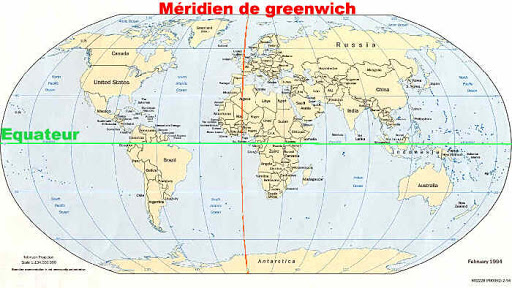
\includegraphics[width=8cm]{ressources/greenwich.jpg}
    \captionof{figure}{Cercles de référence}
    \label{greenwich}
\end{center}
En mathématiques dans un repère en deux dimensions on donne une position en indiquant l'abscisse et l'ordonnée d'un point (figure \ref{coordonnees}).
\begin{center}
    \centering
    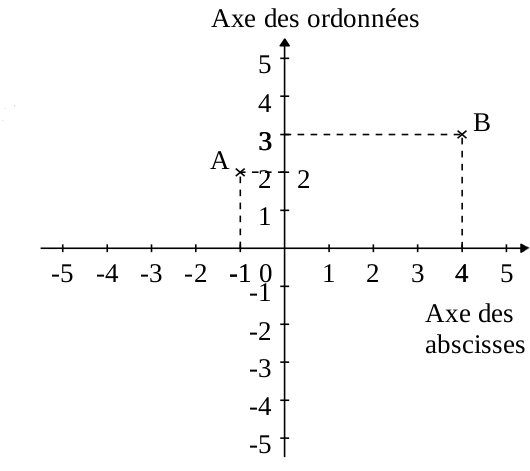
\includegraphics[width=6cm]{ressources/coordonnees.png}
    \captionof{figure}{Coordonnées dans un repère}
    \label{coordonnees}
\end{center}
Pour repérer une position M sur la Terre en trois dimensions on utilise des angles (figure \ref{geoloc}):
\begin{itemize}
    \item sa longitude, angle entre le méridien de Greenwich et le méridien passant par M,
    \item sa latitude, angle entre l’équateur et le parallèle passant par M.
\end{itemize}
\begin{center}
    \centering
    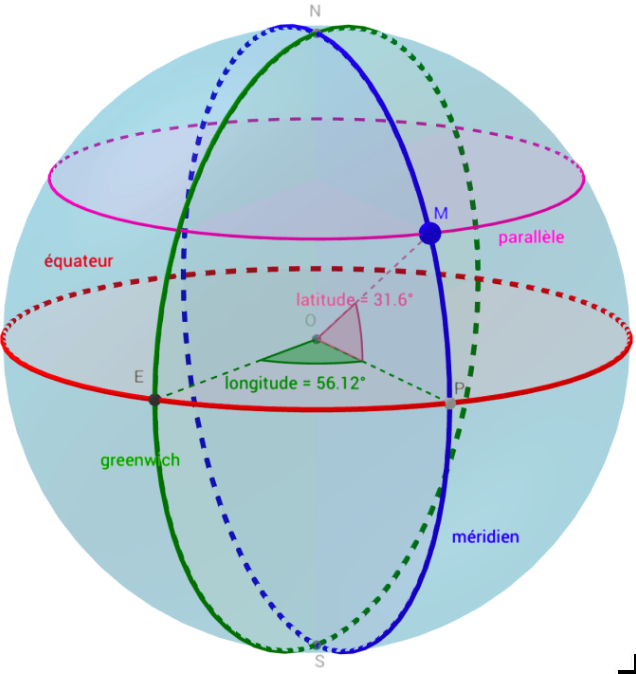
\includegraphics[width=6cm]{ressources/geoloc.png}
    \captionof{figure}{Latitude et longitude}
    \label{geoloc}
\end{center}
Selon les positions par rapport aux axes on indique également les zones (figure \ref{zone}). Ainsi dans la figure \ref{geoloc} les coordonnées du point M sont:
\begin{itemize}
    \item latitude: 31,6°N
    \item longitude: 56,12°E
\end{itemize}
\begin{center}
    \centering
    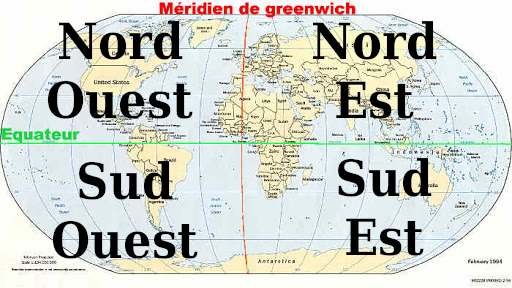
\includegraphics[width=6cm]{ressources/zone.png}
    \captionof{figure}{Zones des latitudes et longitudes}
    \label{zone}
\end{center}
\begin{activite}
    \begin{enumerate}
        \item Dans quelle zone de la figure \ref{zone} est située la France?
        \item Quelle ville de Dordogne est traversée par le méridien de Greenwich (recherche web).
        \item Télécharger et décompresser le dossier \emph{geolocalisation.zip} sur le site \url{https://cviroulaud.github.io}.
        \item Se rendre sur le site \url{https://www.geogebra.org/classic}
        \item Cliquer sur les trois traits horizontaux en haut à droite de la page 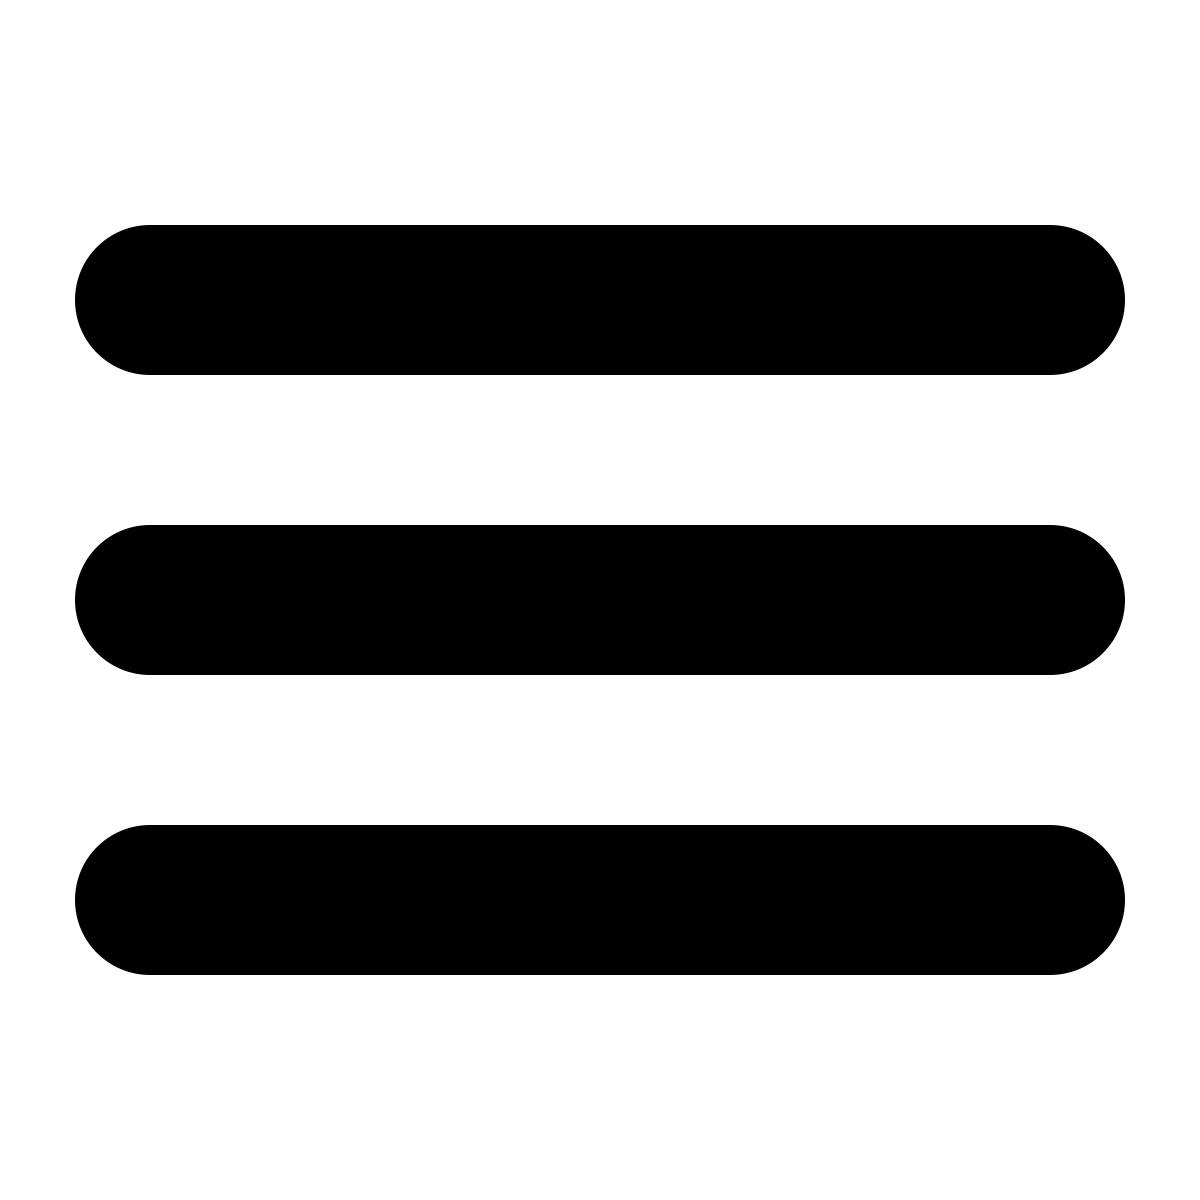
\includegraphics[height=1em]{ressources/hamburger.png} puis \emph{Ouvrir}.
        \item Cliquer sur le dossier à droite 
\includegraphics[height=1em]{ressources/folder.png} puis choisir le fichier \emph{villes.ggb} précédemment téléchargé.
        \item Déplacer le point mobile M pour retrouver les coordonnées des villes et ainsi compléter le tableau ci-dessous. Il faudra également compléter les coordonnées avec N/S/E/O.
              \begin{center}
                  \begin{tabular}{|*{3}{c|}}
                      \hline
                      Noms des villes & Latitudes & Longitudes \\
                      \hline
                                      & 51,5°...  & 0°         \\
                      \hline
                                      & 48,9°...  & 2,3°...    \\
                      \hline
                                      & 40,4°...  & 3,7°...    \\
                      \hline
                                      & 40,6°...  & 116,4°...  \\
                      \hline
                                      & 39,9°...  & 74,1°...   \\
                      \hline
                                      & 56,8°...  & 37,7°...   \\
                      \hline
                  \end{tabular}
              \end{center}
    \end{enumerate}
\end{activite}
\section{Se repérer grâce à des satellites}
\subsection{Principe: la trilatération}
Pour se repérer sur Terre on positionne des satellites artificiels autour du globe (figure \ref{gps0}).
\begin{center}
    \centering
    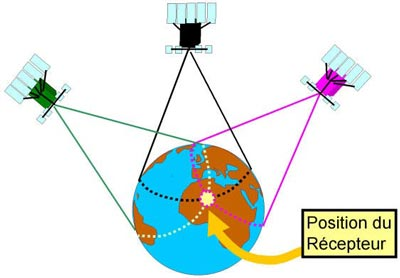
\includegraphics[width=5cm]{ressources/gps0.jpg}
    \captionof{figure}{Un système de satellites}
    \label{gps0}
\end{center}
Chaque satellite envoie sa position très précise dans toutes les directions (figure \ref{gps1}). Le récepteur sur Terre (un smartphone, une montre connectée\dots) est positionné sur la sphère centrée sur le satellite.
\begin{center}
    \centering
    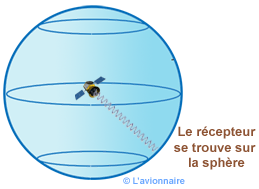
\includegraphics[width=4.5cm]{ressources/gps1.png}
    \captionof{figure}{Signal d'un satellite}

    \label{gps1}
\end{center}
Le récepteur reçoit en même temps la position d'un deuxième satellite. Il est alors quelque part sur \textbf{le cercle} où ces deux sphères se croisent (\ref{gps2}).
\begin{center}
    \centering
    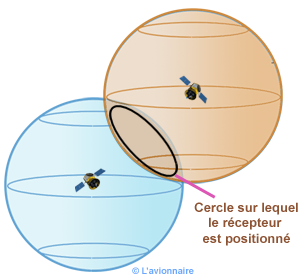
\includegraphics[width=4.5cm]{ressources/gps2.png}
    \captionof{figure}{Intersection des signaux de deux satellites: un cercle}

    \label{gps2}
\end{center}
Le récepteur récupère la position d'un troisième satellite. Les trois sphères ne se croisent qu'en deux points dans l'espace. Un seul de ces points est sur Terre. Le récepteur connaît alors sa position exacte sur Terre (figure \ref{gps3}).
\begin{center}
    \centering
    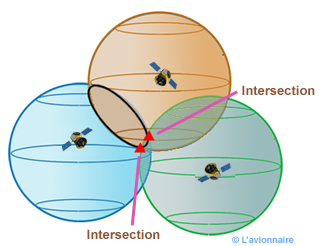
\includegraphics[width=5cm]{ressources/gps3.png}
    \captionof{figure}{Intersection des signaux de trois satellites: deux points}

    \label{gps3}
\end{center}
\begin{aretenir}[Remarque]
En réalité, on utilise un quatrième satellite pour gagner en précision, avoirs des informations sur l'altitude\dots
\end{aretenir}
\subsection{Différents systèmes}
On parle communément de GPS (\emph{Global Positioning System}) car c'est le premier système mis en place par la Défense américaine en 1973. Il utilise 31 satellites. Les informations fournies sont précises à l'ordre du mètre mais cette précision était d'abord réservée à un usage militaire. La population civile ne pouvait obtenir une précision qu'à plusieurs centaines de mètres. Cette limitation a été levée au début des années 2000.
\begin{activite}
\begin{enumerate}
    \item Trouver les noms et caractéristiques des systèmes russes, européens et chinois, concurrents du GPS.
    \item Pour quelles raisons ces pays ont mis en place leur propre système?
\end{enumerate}
\end{activite}
\end{document}